\documentclass{article}
\usepackage{../../Self_Style}

\title{Phys 20 Week 2: Friction}
\author{Zih-Yu Hsieh}
\date{\today}

\begin{document}
\maketitle

\section{Aim for Experiment}

Test out the coefficients of static and kinetic friction of the cart on ramps made of different materials.

\section{Experimental Setup}
Equipments include: Meter stick, tape, masses, mass scale, stand, wooden ramp, clamp, paper, plastic board, protractor, and a cart.

\begin{itemize}
    \item[1.] Fix the stand next to the table.
    \item[2.] Fix the clip onto the wooden ramp, clamp the clip onto the stand, and let one side of the wooden ramp lay on the table. This is used for adjusting the angle of the ramp.
    \item[3.] Fix the protractor's center at the edge of the wooden ramp that's touching the table, which is used to measure the angle.
    \item[4.] Tape the (desired) surface for the experiment (ex: plastic board, paper, etc.) onto the wooden ramp.
\end{itemize}
\begin{figure}[h!]
    \centering
    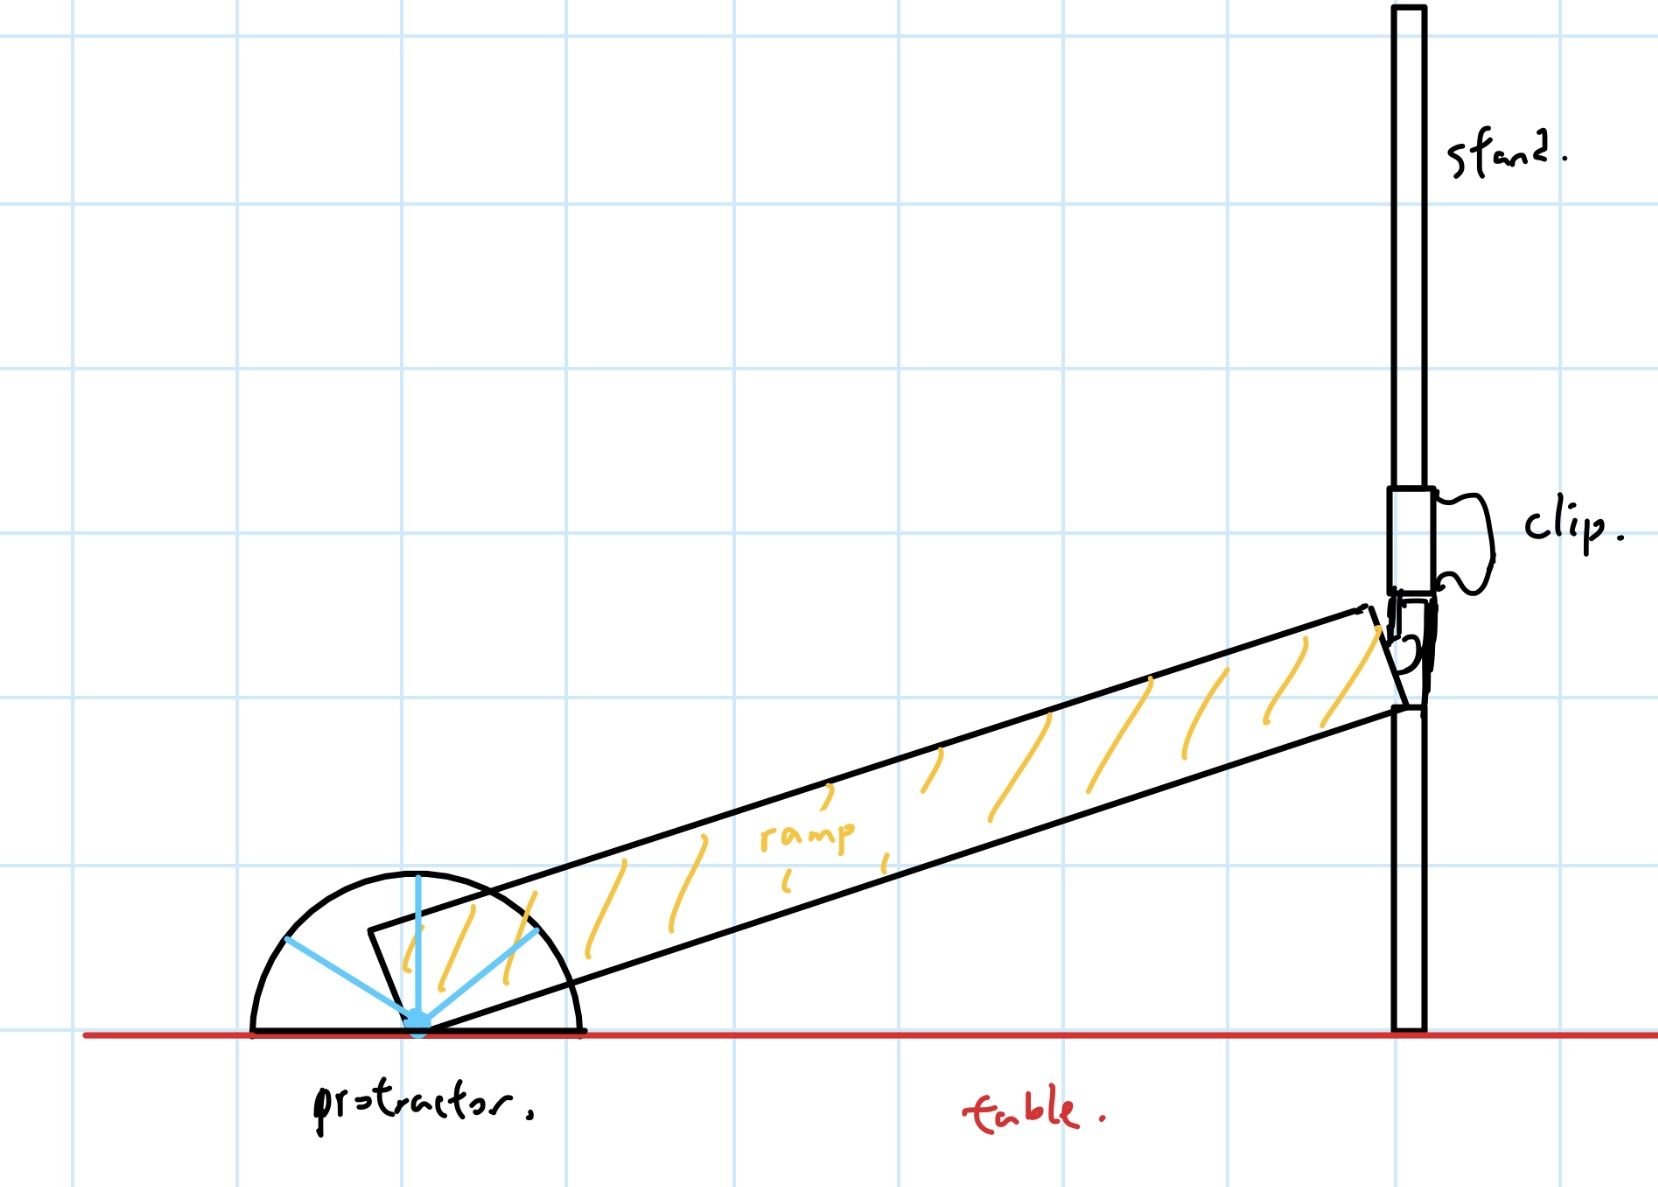
\includegraphics[width=100mm]{setup_sketch.jpg}
    \caption{Sketch of the Experimental Setup}
\end{figure}

\section{Measurement \& Methods of Measure}
For each pair of manipulated variables, we'll do $5$ trials of measurement.

\subsection{Static Friction}
For static friction, the aim is to find the ``Cricial Angle'' when the object starts sliding (or the angle such that gravitational force surpasses static friction).  We'll use the protractor to measure the angle.

To test out the coefficient of static friction for different surfaces (while having the cart sliding on it), we'll fix the mass on the cart (including the cart itself) as $292.1 g$ (or $0.2921$ kg), while varying the material of the surface. In this lab, the materials of the surface include: Wood, Plastic board, and Paper.

Then, to test out the effect of varying mass of the cart on static friction, we'll fix the material of the surface of the ramp (fix as paper), while varying the mass of the cart. Here, the tested masses include: $292.1, 492.5,$ and $576.8$ g. (Or, using kg as standard mass unit, $0.2921, 0.4925,$ and $0.5768$ kg).

\subsection{Kinetic Friction}
For kinetic friction, the aim is to find the total time it takes for the object to travel a fixed distance, which we'll use the timer to measure the elapsed time. If choosing an angle that's strictly greater than the critical angle, ``ideally'' one can assume the kinetic friction is fixed as constant, and as the angle is fixed, the gravitational force also remains constant, hence can assume constant acceleration under this case. Which, to retrieve the acceleration caused by friction, it suffices to know the total acceleration (since other components of accelerations are determined by the mass). 

To test out the coefficient of static friction for a fixed mass and surface, we'll fix the mass as $292.1$ g ($0.2921$ kg), and fix the traveling distance to $27.5$ cm (or $0.275$ m). And, to observe different accelerations, we'll vary the ramp's angle between $15^\circ$, $17.5^\circ$, and $20^\circ$.

\section{Experimental Procedures}

\subsection{Static Friction}
\subsubsection{Varying Materials of the Ramp Surface}
The aim of this section is to test out the critical angle between different materials of the surface of the ramp, while fixing other variables. We'll follow the below procedure:
\begin{itemize}
    \item[1.] Measure a fixed mass of the cart placed on the ramp, and fix a material for the surface of the ramp.
    \item[2.] Put the cart on the flattened ramp, and start slowly increasing the angle of the ramp, by adjusting the position of the clip on the stand.
    \item[3.] When the cart starts to travel (i.e. no longer static), stop increasing the angle of the ramp, and record the angle using the protractor (called \emph{cricial angle}).
    \item[4.] Repeat Step 2 and 3 for five times.
    \item[5.] Keep the mass of the cart fixed, change the material of the surface of the ramp, and redo Step 2 to 4 for each desired material. 
\end{itemize}

\subsubsection{Varying Mass of the Ramp Surface}
The aim of this section is to test out the effect of mass on the critical angle, while fixing other variables. We'll follow the below procedure:
\begin{itemize}
    \item[1.] sFix a material of the surface of the ramp, measure the mass of the cart.
    \item[2.] Put the cart on the flattened ramp, and start slowly increasing the angle of the ramp. 
    \item[3.] When the cart starts to travel, stop increasing the angle of the ramp, and record the angle using the protractor.
    \item[4.] Repeat Step 2 and 3 for five times.
    \item[5.] Keep the material of the surface of the ramp fixed, change the mass of the cart to other values awaited to be tested, and redo Step 2 to 4 for each desired mass.  
\end{itemize}

\subsection{Kinetic Friction}
The aim of this section is to calculate the kinetic friction when the cart is sliding on the ramp. To observe different values, we'll vary the angle of the ramp, while fixing other variables. We'll follow the below procedure:
\begin{itemize}
    \item[1.] Fix the material of the surface of the ramp, measure the fixed mass of the cart, and fix a length on the ramp that the cart would travel each time.
    \item[2.] Set the angle of the ramp to a desired value (where the angle should be larger than the angles found in the section of Static Friction).
    \item[3.] Put the cart on the ramp, and record the time the cart takes to travel the fixed length mentioned in Step 1 (using a timer).
    \item[4.] Repeat Step 2 and 3 for five times.
    \item[5.] Keep the mass of the cart and the material of the surface of teh ramp fixed, change the angle of the ramp to other values awaited to be tested, and redo Step 2 to 4 for each desired angle. 
\end{itemize}

\pagebreak

\section{Collected Data}
\textbf{Static Friction (Varying Surface Material only):}
\begin{figure}[h!]
    \centering
    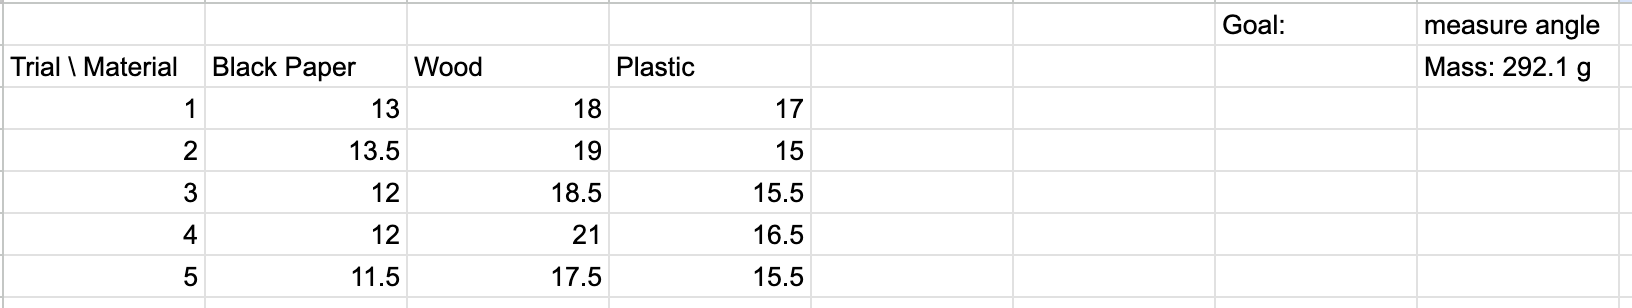
\includegraphics[width=150mm]{static_surface_data.png}

    \hfil

    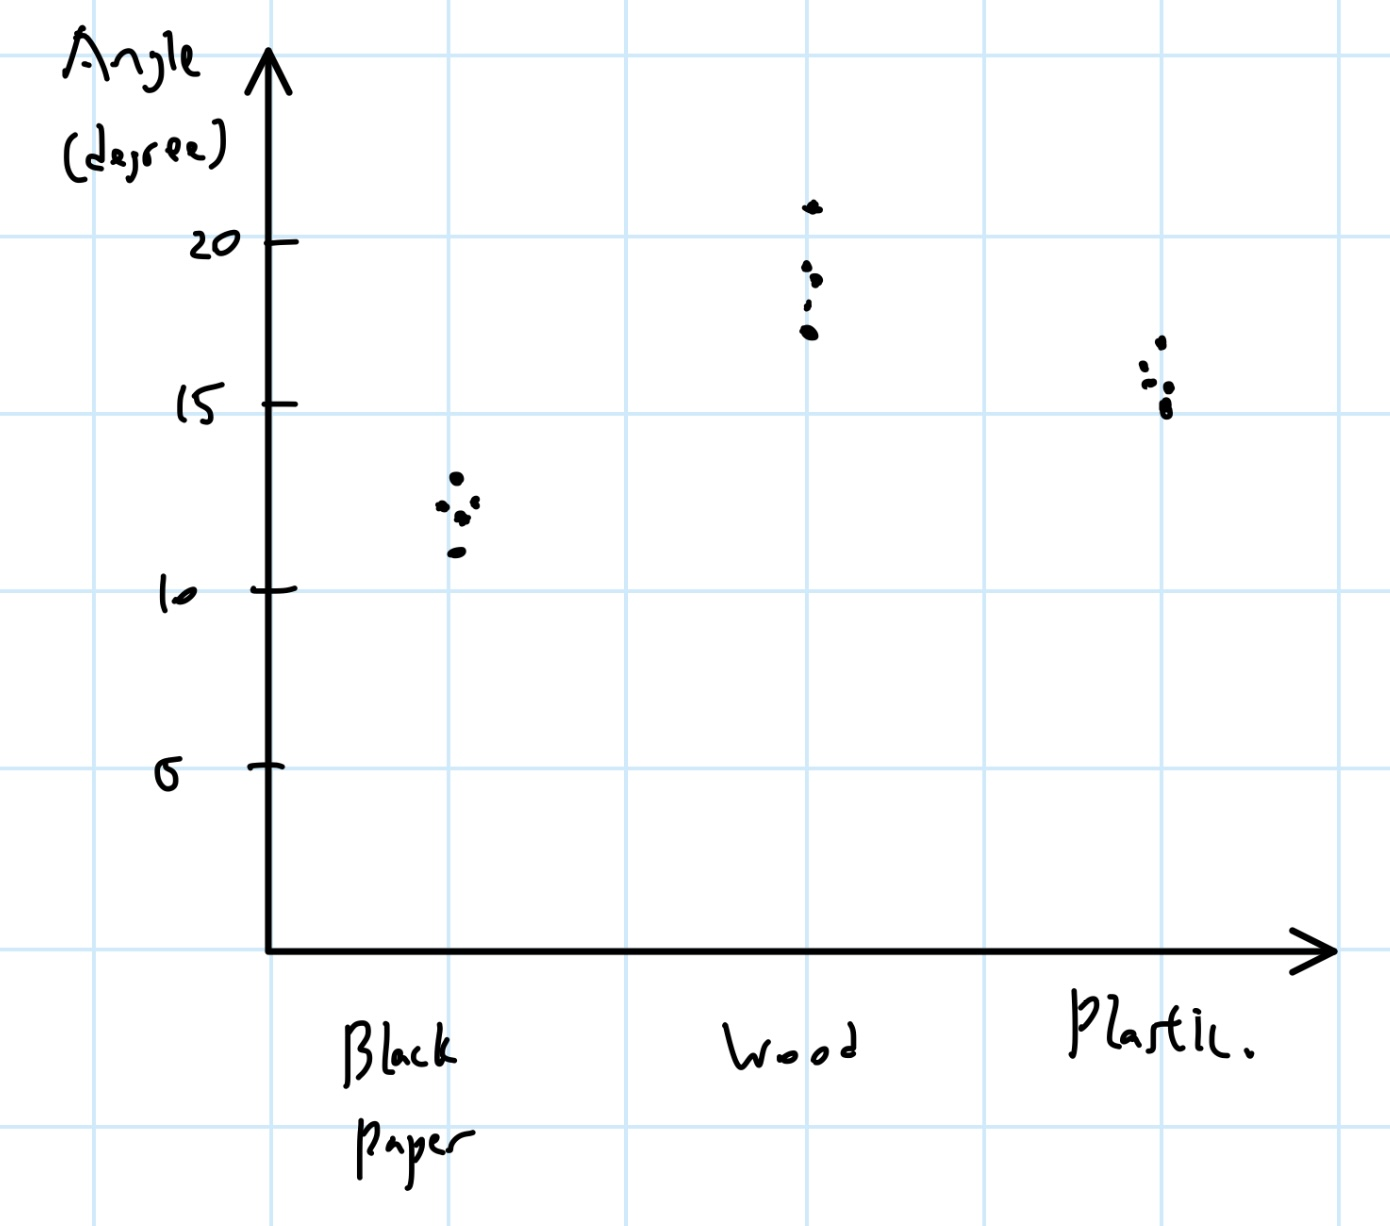
\includegraphics[width=100mm]{static_surface.jpg}
    \caption{Data of Static Friction (varying surface) and Sketch of its Graph}
\end{figure}

\hfil

As an observation, different materials / surface require slightly different angles for the cart to start moving, when fixing the mass. This makes sense as friction should depend on the material / how polished the surface is. 

\pagebreak

\pagebreak

\textbf{Static Friction (Varying Mass only):}

\begin{figure}[h!]
    \centering
    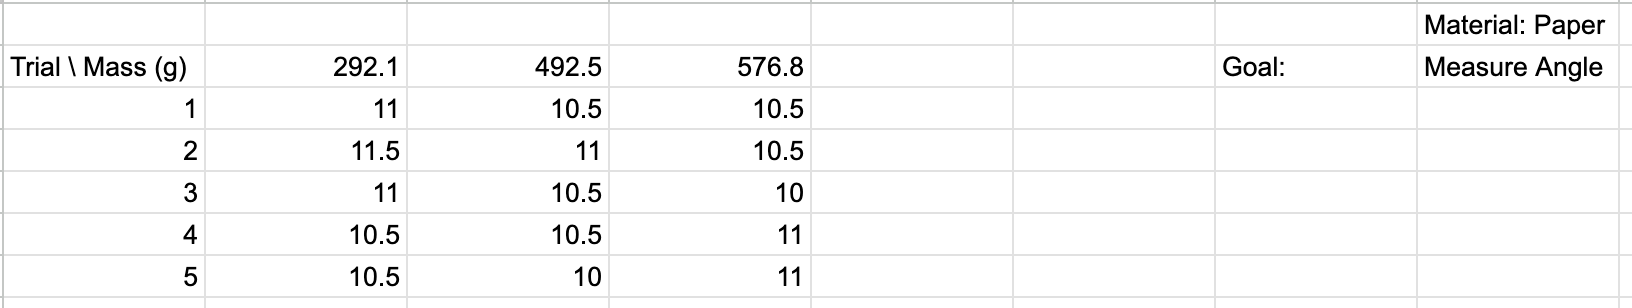
\includegraphics[width=150mm]{static_mass_data.png}

    \hfil

    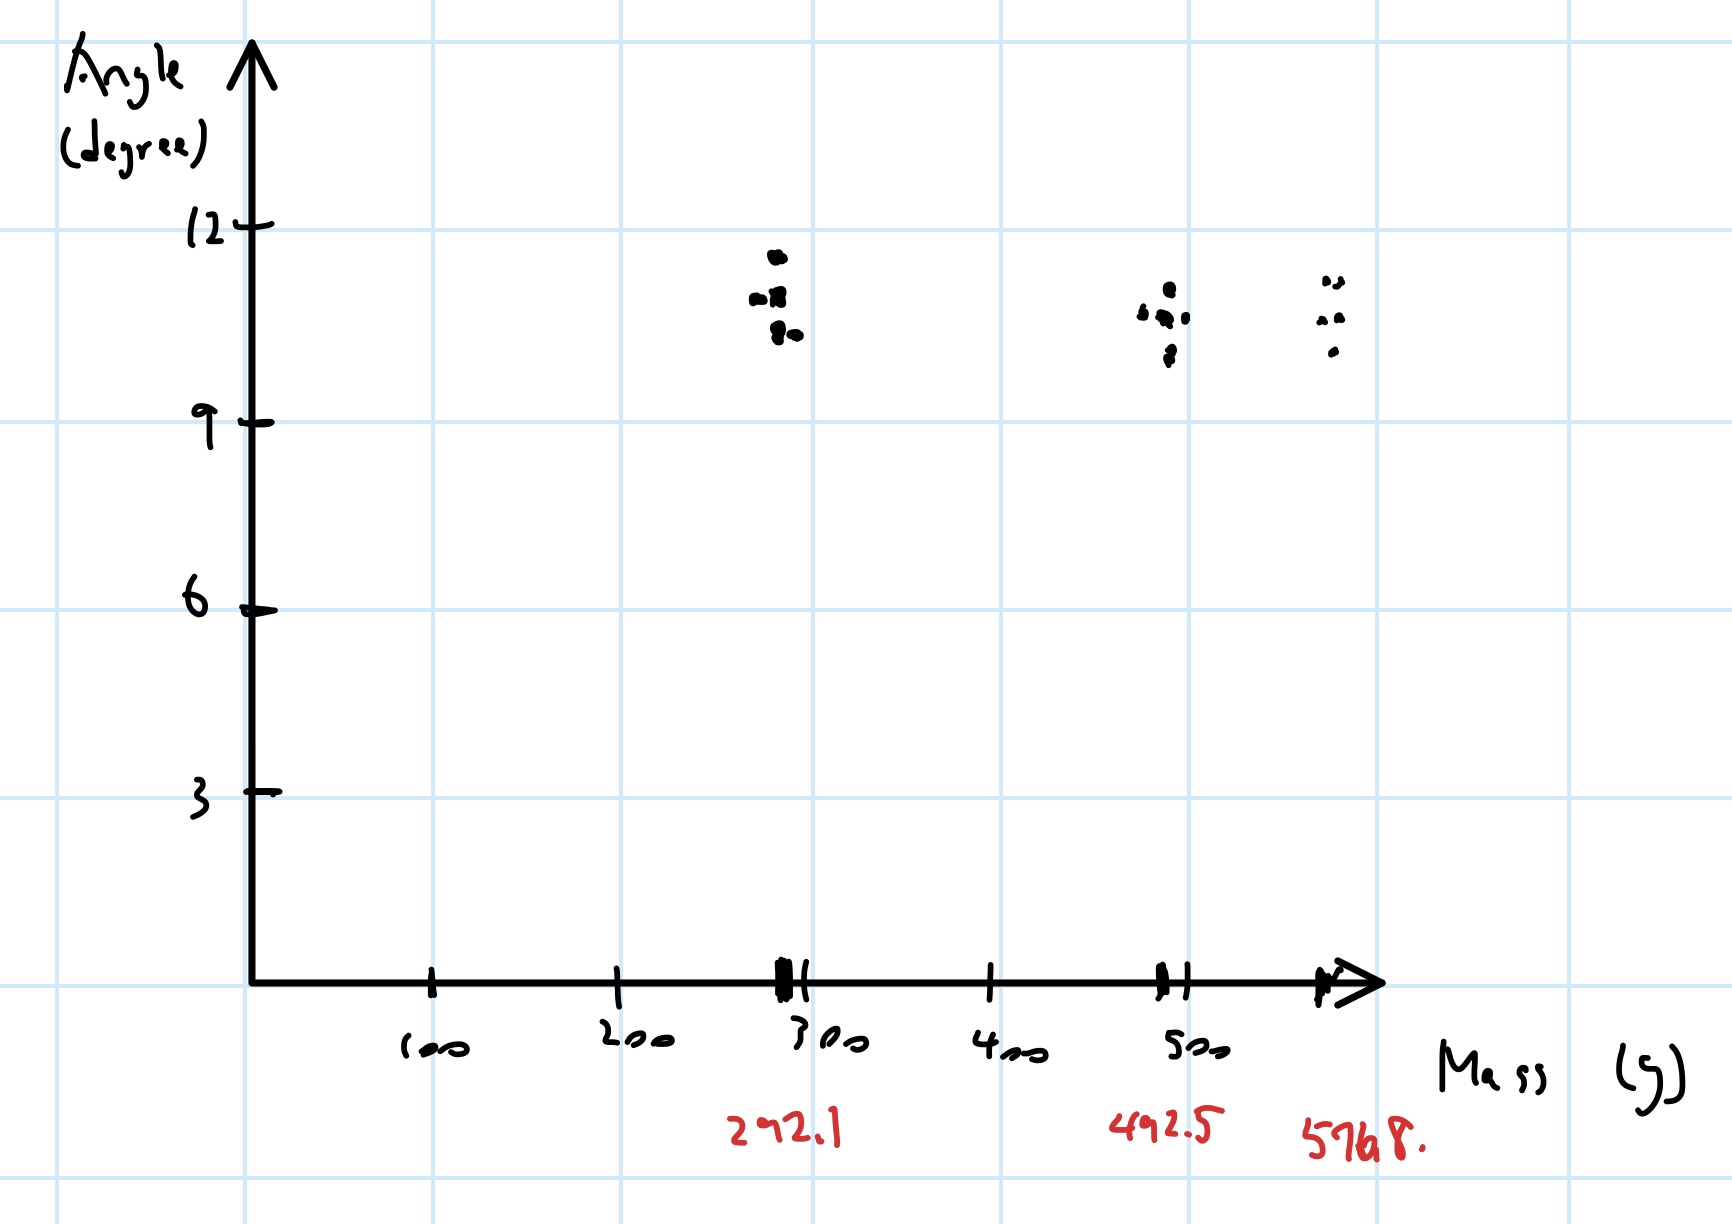
\includegraphics[width=100mm]{static_mass.jpg}
    \caption{Data of Static Friction (varying mass) and Sketch of its Graph}
\end{figure}

\hfil
As an observation, the angle for the cart to start moving didn't vary a lot when changing the mass. This makes sense as friction normally is independent of the mass (based on the formula).

\pagebreak

\pagebreak

\textbf{Kinetic Friction (Varying Ramp Angle only):}
\begin{figure}[h!]
    \centering
    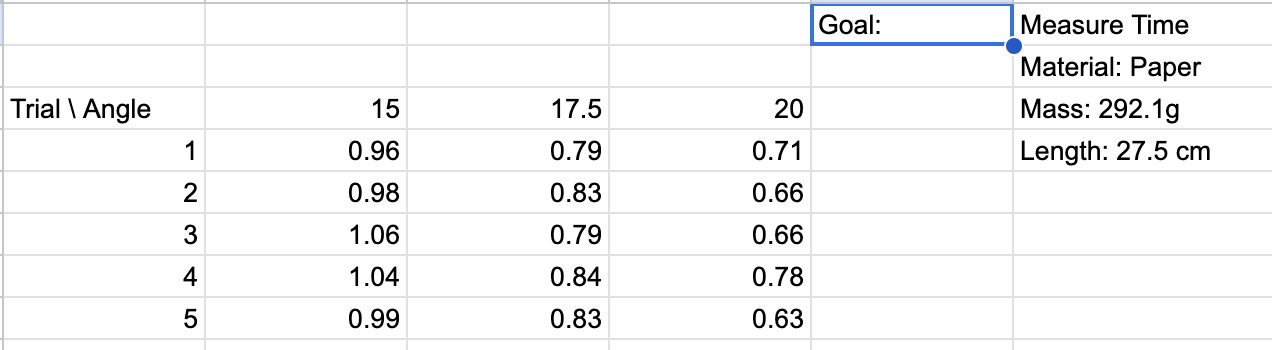
\includegraphics[width=150mm]{kinetic_data.png}

    \hfil

    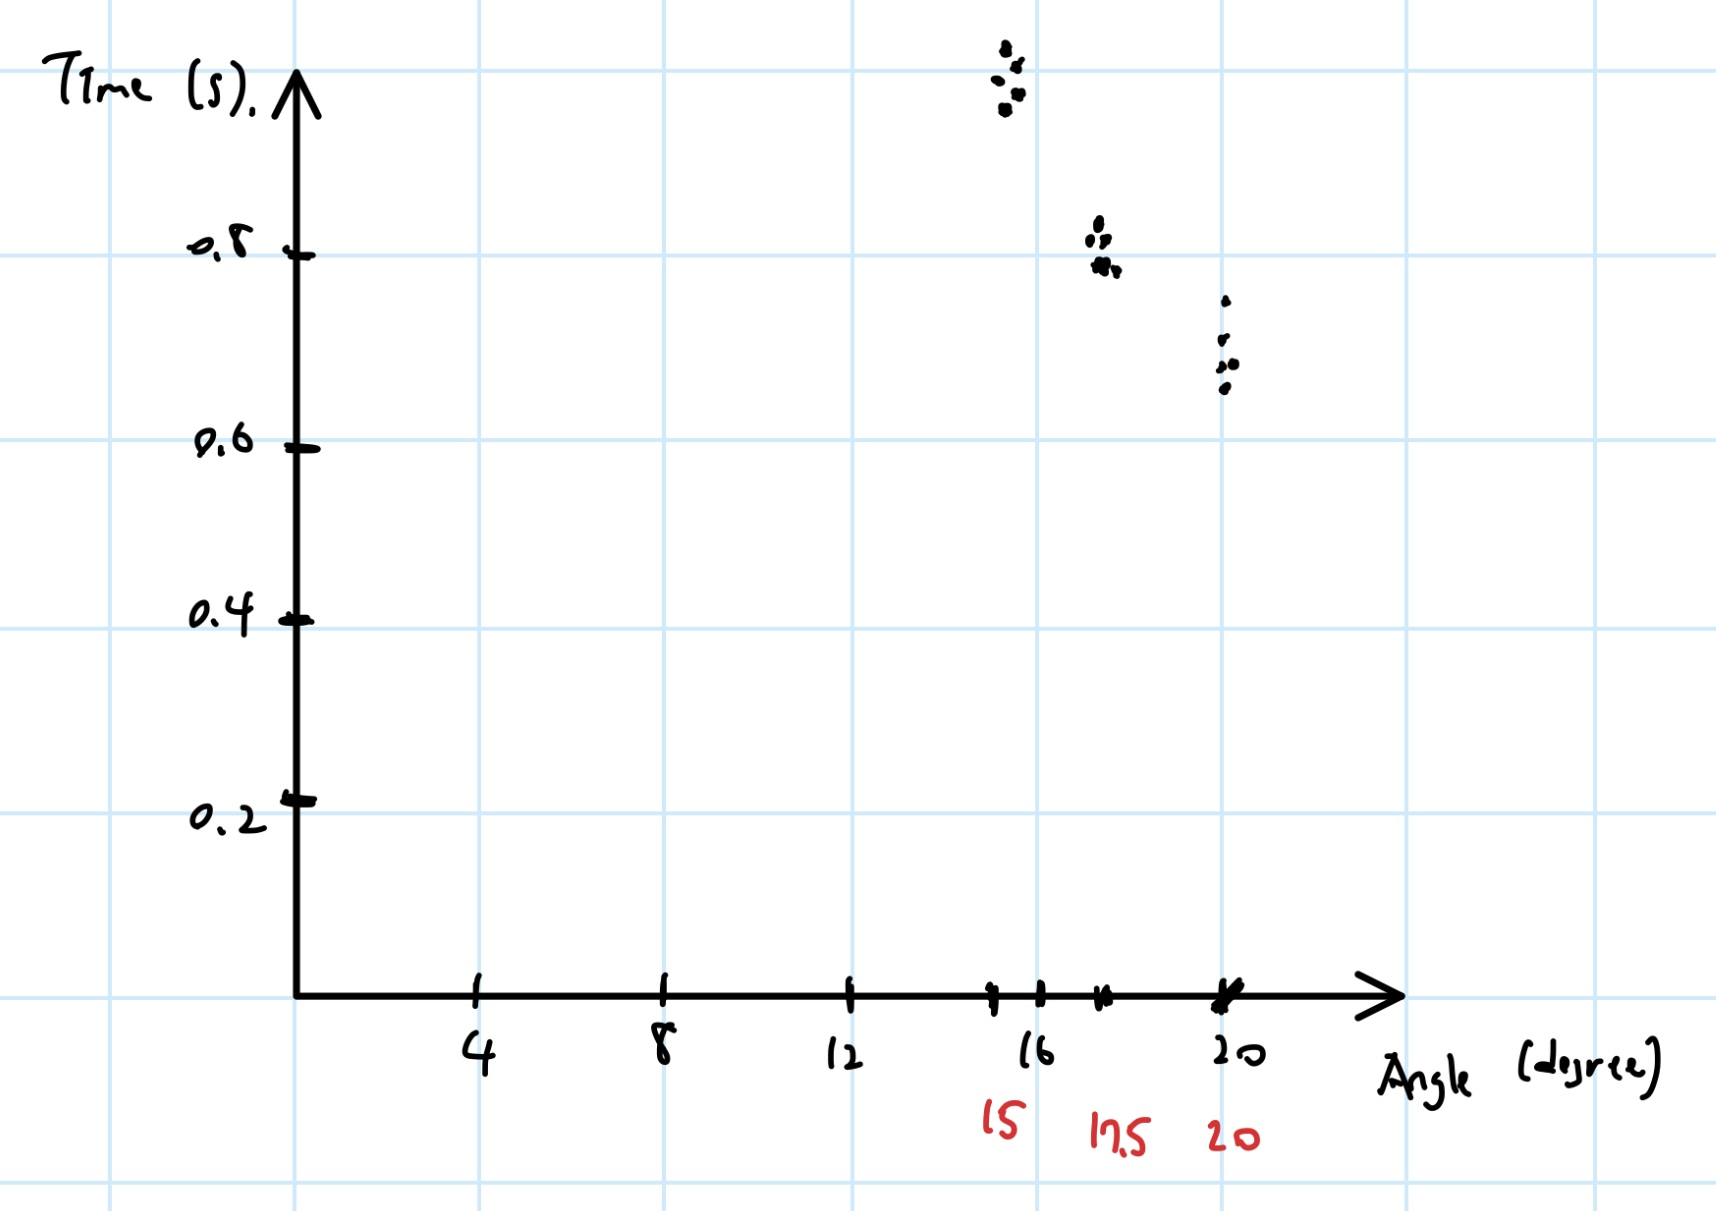
\includegraphics[width=100mm]{kinetic.jpg}
    \caption{Data of Kinetic Friction (varying ramp angle) and Sketch of its Graph}
\end{figure}

\hfil

As an observation, the time it takes for the cart to travel down the ramp is gradually decreasing when we increase the angle of the ramp. This also makes sense as the height of the ramp increases, gravitational force does work more directly on the cart, hence the cart should have larger acceleration (and hence less time to travel through the same distance).


\end{document}